\documentclass[12pt,a4paper]{article}

% ─── Page Layout ───────────────────────────────────────────────────────────────
\usepackage[a4paper, margin=0.8in, headheight=14pt]{geometry}

% ─── Fonts (XeLaTeX) ───────────────────────────────────────────────────────────
\usepackage{fontspec}
\usepackage{unicode-math}
\setmainfont{TeX Gyre Pagella}
\setmonofont[Scale=0.88]{TeX Gyre Cursor}
\setmathfont{Latin Modern Math}

% ─── Packages ──────────────────────────────────────────────────────────────────
\usepackage{xcolor}
\usepackage{colortbl}
\usepackage{titlesec}
\usepackage{enumitem}
\usepackage{tabularx}
\usepackage{booktabs}
\usepackage{array}
\usepackage{amsmath}
\usepackage{tikz}
\usetikzlibrary{shapes.geometric, arrows.meta, positioning, calc, fit, decorations.pathreplacing}
\usepackage{tcolorbox}
\tcbuselibrary{skins, breakable}
\usepackage{hyperref}
\usepackage{fancyhdr}
\usepackage{graphicx}
\usepackage{microtype}
\hyphenpenalty=10000
\exhyphenpenalty=10000
\sloppy
\usepackage{caption}
\usepackage{setspace}
\usepackage{multirow}
\usepackage{tocloft}

% ─── Q&A helper ────────────────────────────────────────────────────────────────
\newcommand{\Q}[1]{\textbf{#1}\par\noindent\ignorespaces}

% ─── Colour Palette ────────────────────────────────────────────────────────────
\definecolor{myred}{RGB}{196,30,58}
\definecolor{mydark}{RGB}{30,30,50}
\definecolor{mygreen}{RGB}{14,120,80}
\definecolor{myteal}{RGB}{0,130,140}
\definecolor{myamber}{RGB}{180,100,0}
\definecolor{mypurple}{RGB}{100,30,160}
\definecolor{mygray}{RGB}{246,247,249}
\definecolor{mgframe}{RGB}{180,185,200}
\definecolor{watermark}{RGB}{145,150,170}
\definecolor{hdrred}{RGB}{250,232,235}
\definecolor{hdrgreen}{RGB}{220,244,233}
\definecolor{hdrteal}{RGB}{220,242,244}
\definecolor{hdramber}{RGB}{253,242,215}
\definecolor{hdrpurple}{RGB}{238,228,255}
\definecolor{hdrgray}{RGB}{238,240,245}
\definecolor{rowalt}{RGB}{250,251,253}

% ─── Section Formatting ────────────────────────────────────────────────────────
\titleformat{\section}
  {\large\bfseries\color{myred}}{\thesection.}{0.5em}{}
  [\vspace{1pt}{\color{myred}\rule{\linewidth}{0.8pt}}]
\titleformat{\subsection}
  {\normalsize\bfseries\color{myteal}}{\thesubsection}{0.5em}{}
\titlespacing*{\section}{0pt}{18pt}{7pt}
\titlespacing*{\subsection}{0pt}{11pt}{4pt}

% ─── Paragraph ─────────────────────────────────────────────────────────────────
\setlength{\parindent}{0pt}
\setlength{\parskip}{4pt}

% ─── TOC Styling ───────────────────────────────────────────────────────────────
\renewcommand{\cfttoctitlefont}{\large\bfseries\color{myred}}
\renewcommand{\cftaftertoctitle}{\par\noindent{\color{myred}\rule{\linewidth}{0.8pt}}}
\setlength{\cftbeforetoctitleskip}{0pt}
\setlength{\cftaftertoctitleskip}{6pt}
\renewcommand{\cftsecfont}{\normalsize\bfseries\color{mydark}}
\renewcommand{\cftsecpagefont}{\normalsize\bfseries\color{mydark}}
\renewcommand{\cftsecleader}{\cftdotfill{\cftdotsep}}
\setlength{\cftbeforesecskip}{7pt}
\renewcommand{\cftsubsecfont}{\small\color{mydark}}
\renewcommand{\cftsubsecpagefont}{\small\color{mydark}}
\setlength{\cftbeforesubsecskip}{3pt}
\setlength{\cftsubsecindent}{1.4em}

% ─── Table helpers ─────────────────────────────────────────────────────────────
\renewcommand{\arraystretch}{1.45}
\setlength{\tabcolsep}{6pt}
\arrayrulecolor{mydark}
\newcolumntype{B}[1]{>{\small\bfseries\raggedright\arraybackslash}m{#1}}
\newcolumntype{Y}{>{\small\raggedright\arraybackslash}X}
\renewcommand{\tabularxcolumn}[1]{m{#1}}

% ─── Header / Footer ───────────────────────────────────────────────────────────
\pagestyle{fancy}
\fancyhf{}
\fancyhead[L]{\small\color{myred}\textbf{OE-EC704C}\;\color{mydark}--- Entrepreneurship}
\fancyhead[R]{\small\color{myteal}\textbf{Module 1 Notes}}
\fancyfoot[C]{\small\color{mydark}\thepage}
\fancyfoot[R]{\small\color{watermark}\textit{\copyright\ Biraj}}
\renewcommand{\headrulewidth}{0.5pt}
\renewcommand{\footrulewidth}{0.3pt}

% ─── Hyperref ──────────────────────────────────────────────────────────────────
\hypersetup{
  colorlinks=true, linkcolor=myteal, urlcolor=myteal,
  pdfauthor={Biraj Sarkar},
  pdftitle={OE-EC704C --- Module 1 Notes}
}

% ─── tcolorbox styles ──────────────────────────────────────────────────────────
\tcbset{
  tikzbox/.style={
    colback=mygray, colframe=mgframe, boxrule=0.6pt, arc=4pt,
    left=8pt, right=8pt, top=6pt, bottom=6pt,
    colbacktitle=mgframe, coltitle=mydark,
    fonttitle=\small\bfseries
  },
  defbox/.style={
    colback=hdrgreen, colframe=mygreen, boxrule=0.8pt, arc=4pt,
    left=9pt, right=9pt, top=6pt, bottom=6pt,
    colbacktitle=mygreen, coltitle=white,
    fonttitle=\small\bfseries
  },
  formulabox/.style={
    colback=hdrteal, colframe=myteal, boxrule=0.8pt, arc=4pt,
    left=9pt, right=9pt, top=7pt, bottom=7pt,
    colbacktitle=myteal, coltitle=white,
    fonttitle=\small\bfseries
  },
  examplebox/.style={
    colback=hdramber, colframe=myamber, boxrule=0.8pt, arc=4pt,
    left=9pt, right=9pt, top=6pt, bottom=6pt,
    colbacktitle=myamber, coltitle=white,
    fonttitle=\small\bfseries
  },
  masonbox/.style={
    colback=hdrpurple, colframe=mypurple, boxrule=0.8pt, arc=4pt,
    left=9pt, right=9pt, top=6pt, bottom=6pt,
    colbacktitle=mypurple, coltitle=white,
    fonttitle=\small\bfseries
  },
  exambox/.style={
    colback=hdrpurple, colframe=mypurple, boxrule=1pt, arc=5pt,
    left=10pt, right=10pt, top=8pt, bottom=8pt,
    colbacktitle=mypurple, coltitle=white,
    fonttitle=\bfseries,
    breakable, title after break={\textbf{Frequently Asked / Viva Questions (contd.)}}}
}
\tcbset{breakable}

% ─── TikZ styles ───────────────────────────────────────────────────────────────
\tikzset{
  block/.style={rectangle, draw=myteal, fill=hdrteal,
    text width=2.4cm, align=center, minimum height=0.95cm,
    font=\small, rounded corners=3pt, line width=0.7pt},
  redblock/.style={rectangle, draw=myred, fill=hdrred,
    text width=2.4cm, align=center, minimum height=0.95cm,
    font=\small, rounded corners=3pt, line width=0.7pt},
  netnode/.style={rectangle, draw=myteal, fill=hdrteal,
    text width=1.5cm, align=center, minimum height=0.8cm,
    font=\small, rounded corners=3pt, line width=0.7pt},
  sumjunc/.style={circle, draw=myamber, fill=hdramber,
    minimum size=0.62cm, font=\small, line width=0.8pt},
  snode/.style={circle, draw=mypurple, fill=hdrpurple,
    minimum size=0.55cm, font=\footnotesize, line width=0.7pt},
  arrow/.style={-Stealth, thick, color=mydark},
  redarrow/.style={-Stealth, thick, color=myred},
  line/.style={thick, color=mydark}
}

% ═══════════════════════════════════════════════════════════════════════════════
\begin{document}
% ═══════════════════════════════════════════════════════════════════════════════

\begin{center}
  {\LARGE\bfseries\color{myred} OE-EC704C --- Entrepreneurship}\\[5pt]
  {\normalsize\color{mydark} Semester VII \quad$\bullet$\quad 3L:0T:0P \quad$\bullet$\quad 3 Credits}\\[3pt]
  {\normalsize\color{myteal}\textbf{Module 1 Exam Notes: Introduction \& Small Scale Industries}}\\[3pt]
  {\small\color{mydark} CGEC \;$|$\; B.Tech ECE (2023--27) \;$|$\; \textit{Biraj Sarkar}}
\end{center}
\vspace{2pt}
\noindent{\color{myred}\rule{\linewidth}{1.5pt}}
\vspace{2pt}

\hypersetup{linkcolor=mydark}
\tableofcontents
\hypersetup{linkcolor=myteal}
\newpage

% ===============================================================================
\section{Industrial Reforms and Policies}
% ===============================================================================

\subsection{New Industrial Policy of 1991 (NIP-91)}
The New Industrial Policy, announced on July 24, 1991, marked a water-shed moment in Indian economic history. It aimed to unshackle the Indian economy from the rigid boundaries of state control (the ``License Raj'') and integrate it with the global market. 

\begin{tcolorbox}[defbox, title={Core Pillars of NIP-91: LPG}]
The policy is structured around three major strategic pillars:
\begin{itemize}[leftmargin=*, itemsep=2pt, topsep=0pt]
  \item \textbf{Liberalization:} Removing government-imposed regulatory hurdles, licensing, and procedural restrictions on businesses.
  \item \textbf{Privatization:} Reducing the role of the public sector by selling government equity in state enterprises (disinvestment) and opening public monopolies to private players.
  \item \textbf{Globalization:} Integrating the domestic economy with the world economy by lowering import tariffs, removing quantitative trade barriers, and allowing foreign capital investments.
\end{itemize}
\end{tcolorbox}

\subsubsection{Key Reform Actions of NIP-91}
\begin{enumerate}[label=\textbf{\arabic*.}, leftmargin=*, itemsep=4pt]
  \item \textbf{Abolition of Industrial Licensing:} Licensing was abolished for all projects, irrespective of investment level, except for 18 strategic and hazardous industries (subsequently reduced to 5, including defense equipment, industrial explosives, hazardous chemicals, tobacco, and alcohol).
  \item \textbf{De-reservation of the Public Sector:} The number of industries reserved exclusively for the public sector was slashed from 17 to 8, and later to just 2 (Atomic Energy and Railway Operations).
  \item \textbf{Reforms in the MRTP Act (1969):} The Monopolies and Restrictive Trade Practices Act was amended to remove the asset threshold limit (previously $\text{Rs. } 100\text{ Crores}$) for pre-entry clearance. Firms no longer required prior approval for expansion, mergers, or establishing new undertakings.
  \item \textbf{Foreign Investment Promotion:} Automatic approval was granted for Foreign Direct Investment (FDI) up to 51\% (later expanded to 100\% in many sectors) in high-priority industries, replacing the case-by-case approval under FERA (1973). The Foreign Investment Promotion Board (FIPB) was established to negotiate and expedite FDI approvals.
  \item \textbf{Public Sector Reforms and Disinvestment:} Government started offloading shares of public sector undertakings (PSUs) to mutual funds, financial institutions, and the public to bring financial discipline and private management efficiency.
\end{enumerate}

% ===============================================================================
\section{Foundations of Entrepreneurship}
% ===============================================================================

\subsection{Meaning and Definition}
\begin{tcolorbox}[defbox, title={Definition of Entrepreneurship}]
\textbf{Entrepreneurship} is the process of identifying, launching, and running a new business venture under conditions of uncertainty, involving the mobilization of resources, innovation, and risk-taking to generate economic value.
\par\vspace{3pt}
An \textbf{Entrepreneur} is a person who perceives a business opportunity, mobilizes the necessary capital, resources, and talent, takes the inherent financial and personal risks, and manages the operations to build a successful enterprise.
\end{tcolorbox}

\subsection{Characteristics of a Successful Entrepreneur}
\begin{itemize}[leftmargin=*, itemsep=3pt]
  \item \textbf{Calculated Risk-Taker:} Willing to take calculated risks based on logical analysis, rather than blind gambling.
  \item \textbf{Innovation (Schumpeterian View):} Introducing new products, new methods of production, opening new markets, finding new raw materials, or establishing new organizational structures.
  \item \textbf{Self-Confidence and Internal Locus of Control:} Believing that they control their own destiny through effort and decision-making, rather than luck or external circumstances.
  \item \textbf{High Achievement Orientation (David McClelland):} Driven by a strong need for achievement ($\text{n-Ach}$), taking personal responsibility to solve complex problems and meet high standards.
  \item \textbf{Flexibility and Resilience:} Ability to adapt to market feedback and bounce back from operational setbacks or project failures.
\end{itemize}

\subsection{Intrapreneur vs. Entrepreneur vs. Manager}
\par\noindent
{\renewcommand{\arraystretch}{1.5}%
\begin{tabularx}{\linewidth}{|B{2.5cm}|Y|Y|Y|}\hline
\multicolumn{1}{|>{\centering\arraybackslash}m{2.5cm}|}{\textbf{Parameter}} &
\multicolumn{1}{>{\centering\arraybackslash}Y|}{\textbf{Entrepreneur}} &
\multicolumn{1}{>{\centering\arraybackslash}Y|}{\textbf{Intrapreneur}} &
\multicolumn{1}{>{\centering\arraybackslash}Y|}{\textbf{Manager}} \\
\hline
\textbf{Status} & Owner of the independent enterprise. & Employee within a large corporate organization. & Salaried employee in an organization. \\
\hline
\textbf{Risk-Taking} & Bears entire financial and personal risk. & Minimal financial risk; company bears the loss. & Bears no financial risk; performance-related risk only. \\
\hline
\textbf{Primary Goal} & Create value, innovation, independence. & Develop new business lines for the corporate parent. & Maintain status quo, meet targets, administer processes. \\
\hline
\textbf{Funding} & Mobilizes capital from personal savings, debt, or equity. & Provided entirely by the corporate employer. & Operates within approved department budgets. \\
\hline
\textbf{Reward} & Business profits and equity appreciation. & Salary, bonuses, promotions, or project commissions. & Fixed salary, perks, and performance incentives. \\
\hline
\end{tabularx}
}

% ===============================================================================
\section{Small Scale Industries (SSI) in India}
% ===============================================================================

\subsection{Definition and Classification}
Small Scale Industries (SSIs) are industrial undertakings in which the investment in plant and machinery or equipment does not exceed a specified threshold limit. Under the revised MSME Act of 2020, India transitioned from separate manufacturing/services criteria to a composite classification based on investment and annual turnover:

\begin{tcolorbox}[defbox, title={Revised Composite MSME Classification (Post-2020)}]
\renewcommand{\arraystretch}{1.3}
\begin{tabularx}{\linewidth}{l B{3.8cm} Y}
\textbf{Enterprise Class} & \textbf{Investment in Plant/Machinery} & \textbf{Annual Turnover} \\
\midrule
\textbf{Micro} & $\le \text{Rs. } 1 \text{ Crore}$ & $\le \text{Rs. } 5 \text{ Crores}$ \\
\textbf{Small (SSI)} & $\le \text{Rs. } 10 \text{ Crores}$ & $\le \text{Rs. } 50 \text{ Crores}$ \\
\textbf{Medium} & $\le \text{Rs. } 50 \text{ Crores}$ & $\le \text{Rs. } 250 \text{ Crores}$ \\
\end{tabularx}
\end{tcolorbox}

\subsection{Role and Growth of SSI in the Indian Economy}
Small Scale Industries form the backbone of the Indian manufacturing sector:
\begin{itemize}[leftmargin=*, itemsep=3pt]
  \item \textbf{Employment Generation:} SSIs are highly labor-intensive, requiring less capital per worker compared to large-scale units. They are the second-largest employer after agriculture.
  \item \textbf{Contribution to GDP \& Manufacturing:} SSIs contribute approximately 30\% of India's GDP and nearly 45\% of the country's total manufacturing output.
  \item \textbf{Regional Economic Balance:} Because they can be set up easily in semi-urban and rural areas, they prevent migration to cities and reduce regional economic disparities.
  \item \textbf{Export Promotion:} SSIs account for nearly 40\% of India's direct and indirect exports (handicrafts, textiles, leather, software, and light engineering goods).
\end{itemize}

\subsection{Dearth of Entrepreneurial Talent in India}
Despite having a large young population, India has traditionally faced a shortage of high-impact entrepreneurial talent due to several structural factors:
\begin{enumerate}[label=\textbf{\alph*.}, leftmargin=*, itemsep=2.5pt]
  \item \textbf{Socio-Cultural Factors:} Deep-rooted societal preference for secure jobs (civil services, corporate jobs) over high-risk business ventures. Failure is often stigmatized socially.
  \item \textbf{Rote-Based Education System:} The mainstream academic system emphasizes memorization, exams, and grades rather than innovation, creative thinking, and risk-taking.
  \item \textbf{Financial Constraints:} Lack of seed capital, venture funding in early stages, and high collateral requirements by conventional banks discourage first-generation founders.
  \item \textbf{Bureaucratic Red Tape:} Complex compliance procedures, multiple tax filings, labor laws, and licensing delays historically made starting and running a business painful.
\end{enumerate}

\subsection{Incentives and Benefits for SSIs \& New Entrepreneurs}
To support new entrepreneurs and expand the SSI footprint, the Government of India provides a range of financial and administrative incentives:

\begin{tcolorbox}[formulabox, title={Key Incentives \& Support Programs}]
\begin{itemize}[leftmargin=*, itemsep=2pt, topsep=0pt]
  \item \textbf{Priority Sector Lending (PSL):} Commercial banks are mandated to allocate a fixed percentage of their net lending to MSMEs at lower interest rates.
  \item \textbf{Credit Guarantee Fund Trust for Micro and Small Enterprises (CGTMSE):} Collateral-free loans up to $\text{Rs. } 2\text{ Crores}$ are guaranteed by the trust, reducing risk for commercial banks.
  \item \textbf{Tax Holiday and Concessions:} New manufacturing units under MSME schemes receive income tax exemptions for initial years and lower corporate tax rates.
  \item \textbf{Market Assistance \& Subsidies:} Subsidies on ISO certification cost (up to 75\%), patent registration costs (up to 50\%), and free participation in international trade fairs.
  \item \textbf{Udyam Portal Registration:} A simplified, paperless portal providing immediate MSME certification using Aadhaar card numbers, facilitating fast loan processing and concession claims.
\end{itemize}
\end{tcolorbox}

\subsubsection{Institutional Support Framework}
\begin{itemize}[leftmargin=*, itemsep=3pt]
  \item \textbf{SIDBI (Small Industries Development Bank of India):} The principal financial institution for refinancing and financing MSMEs.
  \item \textbf{DIC (District Industries Centre):} Located in every district, DICs serve as single-window agencies to provide licenses, raw materials, land allotments, and advice to new local entrepreneurs.
  \item \textbf{NSIC (National Small Industries Corporation):} Helps SSIs in marketing, raw material procurement, and technology upgradation.
  \item \textbf{MSME-DI (MSME Development Institute):} Conducts entrepreneurship development programs (EDPs) and technical consultancy services.
\end{itemize}

% ===============================================================================
\section{Operational Procedure to Start an SSI}
% ===============================================================================

Starting a Small Scale Industry in India involves a structured sequence of planning, legal, financial, and operational steps. The complete process is mapped below:

\begin{tcolorbox}[tikzbox, title={Step-by-Step Procedure to Start an SSI}]
\centering
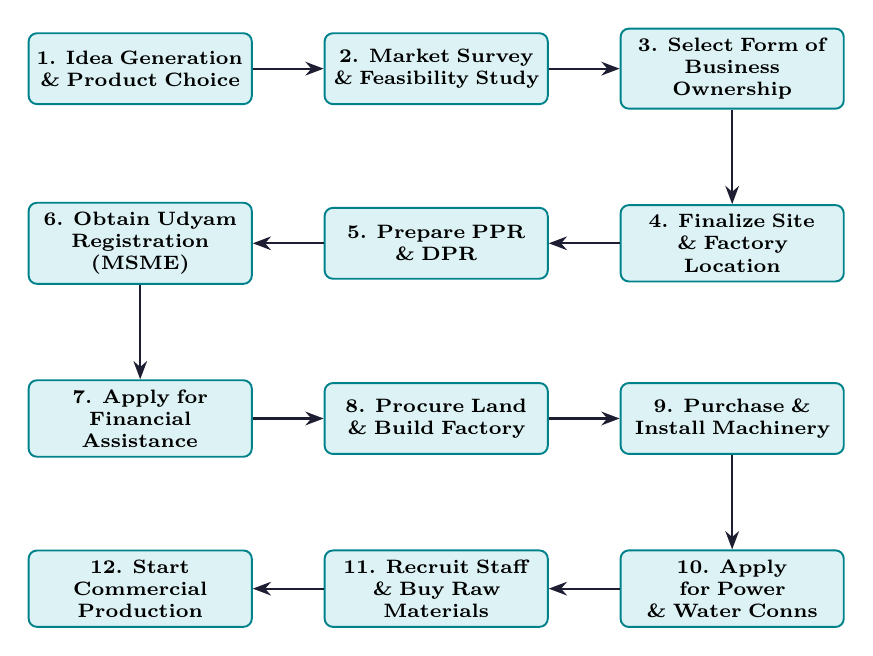
\begin{tikzpicture}[
  node distance=1.0cm and 0.9cm,
  block/.style={rectangle, draw=myteal, fill=hdrteal, text width=2.6cm, align=center, minimum height=0.9cm, font=\scriptsize\bfseries, rounded corners=3pt, line width=0.7pt},
  arrow/.style={-Stealth, thick, color=mydark}
]
  % Row 1
  \node[block] (s1) {1. Idea Generation \\ \& Product Choice};
  \node[block, right=of s1] (s2) {2. Market Survey \\ \& Feasibility Study};
  \node[block, right=of s2] (s3) {3. Select Form of \\ Business Ownership};
  
  % Row 2
  \node[block, below=1.2cm of s3] (s4) {4. Finalize Site \\ \& Factory Location};
  \node[block, left=of s4] (s5) {5. Prepare PPR \\ \& DPR};
  \node[block, left=of s5] (s6) {6. Obtain Udyam \\ Registration (MSME)};
  
  % Row 3
  \node[block, below=1.2cm of s6] (s7) {7. Apply for \\ Financial Assistance};
  \node[block, right=of s7] (s8) {8. Procure Land \\ \& Build Factory};
  \node[block, right=of s8] (s9) {9. Purchase \& \\ Install Machinery};
  
  % Row 4
  \node[block, below=1.2cm of s9] (s10) {10. Apply for Power \\ \& Water Conns};
  \node[block, left=of s10] (s11) {11. Recruit Staff \\ \& Buy Raw Materials};
  \node[block, left=of s11] (s12) {12. Start Commercial \\ Production};

  % Connective paths
  \draw[arrow] (s1) -- (s2);
  \draw[arrow] (s2) -- (s3);
  \draw[arrow] (s3) -- (s4);
  \draw[arrow] (s4) -- (s5);
  \draw[arrow] (s5) -- (s6);
  \draw[arrow] (s6) -- (s7);
  \draw[arrow] (s7) -- (s8);
  \draw[arrow] (s8) -- (s9);
  \draw[arrow] (s9) -- (s10);
  \draw[arrow] (s10) -- (s11);
  \draw[arrow] (s11) -- (s12);
\end{tikzpicture}
\end{tcolorbox}

\subsubsection{Details of the Process Steps}
\begin{enumerate}[label=\textbf{\arabic*.}, leftmargin=*, itemsep=3.5pt]
  \item \textbf{Idea Generation and Product Selection:} Identifying market demands or import substitutes. The entrepreneur selects a product based on their expertise, raw material availability, and market needs.
  \item \textbf{Market Survey and Feasibility Study:} Conducting surveys to estimate demand, competitive intensity, pricing points, and manufacturing costs.
  \item \textbf{Form of Business Ownership:} Deciding whether to register as a Sole Proprietorship, Partnership, Limited Liability Partnership (LLP), or a Private Limited Company.
  \item \textbf{Location and Site Selection:} Selecting a site with proximity to raw materials, labor, transport facilities, and markets, preferably in industrial estates.
  \item \textbf{Prepare PPR \& DPR:} Drafting a Preliminary Project Report (PPR) for initial clearances and a Detailed Project Report (DPR) to secure bank funding.
  \item \textbf{Udyam Registration:} Obtaining the official MSME registration online, which generates an Udyam Registration Number (URN).
  \item \textbf{Apply for Financing:} Submitting the DPR to banks or state financial corporations to secure term loans (for machinery) and working capital loans.
  \item \textbf{Land \& Building Development:} Registering land and constructing the factory layout according to local municipality and safety regulations.
  \item \textbf{Machinery and Equipment Procurement:} Ordering plant machinery from reliable vendors.
  \item \textbf{Utilities Connection:} Applying for industrial electrical power load from the state electricity board and water connections from the municipal board.
  \item \textbf{Workforce \& Material Procurement:} Recruiting technical staff and line workers, and placing orders for initial raw material batches.
  \item \textbf{Commercial Production:} Running trial batches to calibrate machinery and starting commercial manufacture.
\end{enumerate}

\newpage

% ===============================================================================
% MANDATORY QUICK REVISION PAGE
% ===============================================================================
\begin{center}
  {\large\bfseries\color{myred} Quick Revision --- Module 1}\\[3pt]
  {\small\color{mydark} Introduction \& Small Scale Industries $|$ OE-EC704C}
\end{center}
\noindent{\color{myred}\rule{\linewidth}{1.2pt}}
\vspace{4pt}

\begin{tcolorbox}[formulabox, title={\textbf{Key Concepts at a Glance}}]
\renewcommand{\arraystretch}{1.3}
\begin{tabularx}{\linewidth}{B{4.0cm} X}
NIP-91 & Liberalization, Privatization, and Globalization (LPG) reform model. \\
Composite Criteria 2020 & MSME classification combining Investment AND Turnover thresholds. \\
SSI (Small Enterprise) & Investment limit $\le \text{Rs. } 10 \text{ Crores}$ AND Annual Turnover $\le \text{Rs. } 50 \text{ Crores}$. \\
CGTMSE & Scheme offering collateral-free credit guarantee for MSME loans. \\
Udyam Portal & Paperless Aadhaar-linked registration system for Indian MSMEs. \\
n-Ach (Achievement Needs) & Key psychological driver of entrepreneurial risk-taking behavior. \\
\end{tabularx}
\end{tcolorbox}

\begin{tcolorbox}[defbox, title={\textbf{One-Line Definitions}}]
\begin{itemize}[leftmargin=*, itemsep=2.5pt, topsep=0pt]
  \item \textbf{Entrepreneurship:} Act of identifying business ideas, mobilizing capital, taking risk, and establishing a venture.
  \item \textbf{Intrapreneurship:} Act of driving innovation and new business lines within the safe environment of an established corporate firm.
  \item \textbf{Liberalization:} Deregulating industry by removing license limits and procedural bottlenecks.
  \item \textbf{Privatization:} Transferring ownership or operation of public enterprise assets to private ownership.
  \item \textbf{Small Scale Industry (SSI):} Enterprise with plant/machinery investment up to $10 \text{ Crores}$ and turnover up to $50 \text{ Crores}$.
  \item \textbf{District Industries Centre (DIC):} Centralized district-level agency providing support and licenses to local micro/small units.
  \item \textbf{Detailed Project Report (DPR):} Detailed feasibility plan and financial forecast document used to secure bank capital.
\end{itemize}
\end{tcolorbox}

\begin{tcolorbox}[exambox, title={\textbf{Frequently Asked / Viva Questions}}]
\begin{enumerate}[topsep=0pt, label=\textbf{Q\arabic*.}, itemsep=5pt]
  \item \Q{What were the main changes introduced in the Industrial Licensing policy of 1991?}
    Industrial licensing was completely abolished for all new projects, regardless of investment scale, except for five strategic or hazardous sectors (Defense, Explosives, Chemicals, Tobacco, Alcohol).
  \item \Q{How are Small Scale Industries defined post-2020 in India?}
    Under the 2020 composite criteria, a Small Enterprise (SSI) has an investment in plant/machinery of up to $\text{Rs. } 10\text{ Crores}$ and an annual turnover not exceeding $\text{Rs. } 50\text{ Crores}$.
  \item \Q{Differentiate between an Entrepreneur and an Intrapreneur.}
    An entrepreneur operates independently, mobilizes external capital, and bears all financial and personal risks. An intrapreneur behaves like an entrepreneur but works within a corporate system, utilizing corporate resources without personal financial exposure.
  \item \Q{State the contribution of SSIs to the Indian economy.}
    SSIs account for approximately 30\% of India's GDP, 45\% of total manufacturing output, and 40\% of direct/indirect exports, while being the second largest employer after agriculture.
  \item \Q{Identify the major causes for the dearth of entrepreneurial talent in India.}
    The major causes are socio-cultural stigma against business failure, a rote-learning oriented academic system that discourages critical thinking, limited access to early-stage collateral-free seed capital, and historical bureaucratic bottlenecks.
  \item \Q{What is the CGTMSE scheme?}
    The Credit Guarantee Fund Trust for Micro and Small Enterprises is a scheme that provides credit guarantees to commercial banks, allowing MSMEs to secure collateral-free loans up to $\text{Rs. } 2\text{ Crores}$.
  \item \Q{List the primary steps to start a Small Scale Industry.}
    Idea generation $\rightarrow$ Feasibility survey $\rightarrow$ Ownership structure $\rightarrow$ Location $\rightarrow$ PPR/DPR drafting $\rightarrow$ Udyam registration $\rightarrow$ Raising finance $\rightarrow$ Land/Factory development $\rightarrow$ Machine installation $\rightarrow$ Utility connections $\rightarrow$ Material procurement $\rightarrow$ Commercial production.
  \item \Q{What are District Industries Centres (DICs)?}
    DICs are district-level single-window clearance and support agencies that assist local entrepreneurs in obtaining licenses, raw material quotas, subsidies, and credit.
  \item \Q{Explain the MRTP Act change in NIP-91.}
    NIP-91 abolished the asset threshold limit of $\text{Rs. } 100\text{ Crores}$ for MRTP companies, allowing them to expand, merge, or establish new units without prior government approvals.
  \item \Q{What is FIPB and its purpose?}
    The Foreign Investment Promotion Board was established to process and approve foreign direct investment proposals in India that fell outside the automatic approval route.
  \end{enumerate}
\end{tcolorbox}

\end{document}
